\documentclass{scrartcl}
\usepackage[utf8]{inputenc}
\usepackage[T1]{fontenc}
\usepackage[finnish]{babel}
\usepackage{graphicx}
\usepackage{amssymb}
\usepackage{setspace}
\usepackage{amsthm}

\title{Van Aubelin lause}
\author{Kandidaatintutkielma\\Maria Larionova}
\date{\today}

\begin{document}
\maketitle
\pagebreak
\tableofcontents
\pagebreak


\section{Johdanto}
Van Aubelin lause käsittelee nelikulmioiden sivuun piirrettävien neliöiden ominaisuutta. Sen mukaan minkä tahansa nelikulmion jokaista sivua kohti piirretään neliö, jonka sivujen pituudet ovat saman pituisia kuin sen nelikulmion sivun pituus, johon neliö yhtyy. Tällaisten neliöiden keskipisteistä piirretään vastakkaiseen neliön keskipisteeseen jana. Van Aubelin lauseen mukaan, nämä janat ovat yhtä pitkiä ja leikkaavat toisensa kohtisuorassa. 

Lause on nimetty H. H. van Aubelin mukaan, joka julkaisi todistuksen vuonna 1878.

\pagebreak
\section{Esitiedot}
Todistuksessa tulemme käyttämään yhteneviä kolmiota, niiden määritelmää ja ominaisuuksia, nämä tiedot oletan esitiedoiksi. Tämän lisäksi käytämme kolmion sivuille piirrettyjen neliöiden ominaisuutta. Koska tämä ei ole niin itsestään selvää niin avaan lausetta ja todistan sen lyhyesti. Tässä todistuksessa oletan esitiedoiksi kolmion sivujen keskipisteet yhdistävän janan määritelmän ja sen ominaisuudet.

\medskip
\textbf{Lause:} Kolmion kahdelle sivulle piirrettyjen neliöiden keskipisteestä kolmion kolmannen sivun keskipisteeseen piirrettyjen janojen pituus on yhtä suuri sekä niiden väliin muodostuu suorakulma.
\begin{center}
    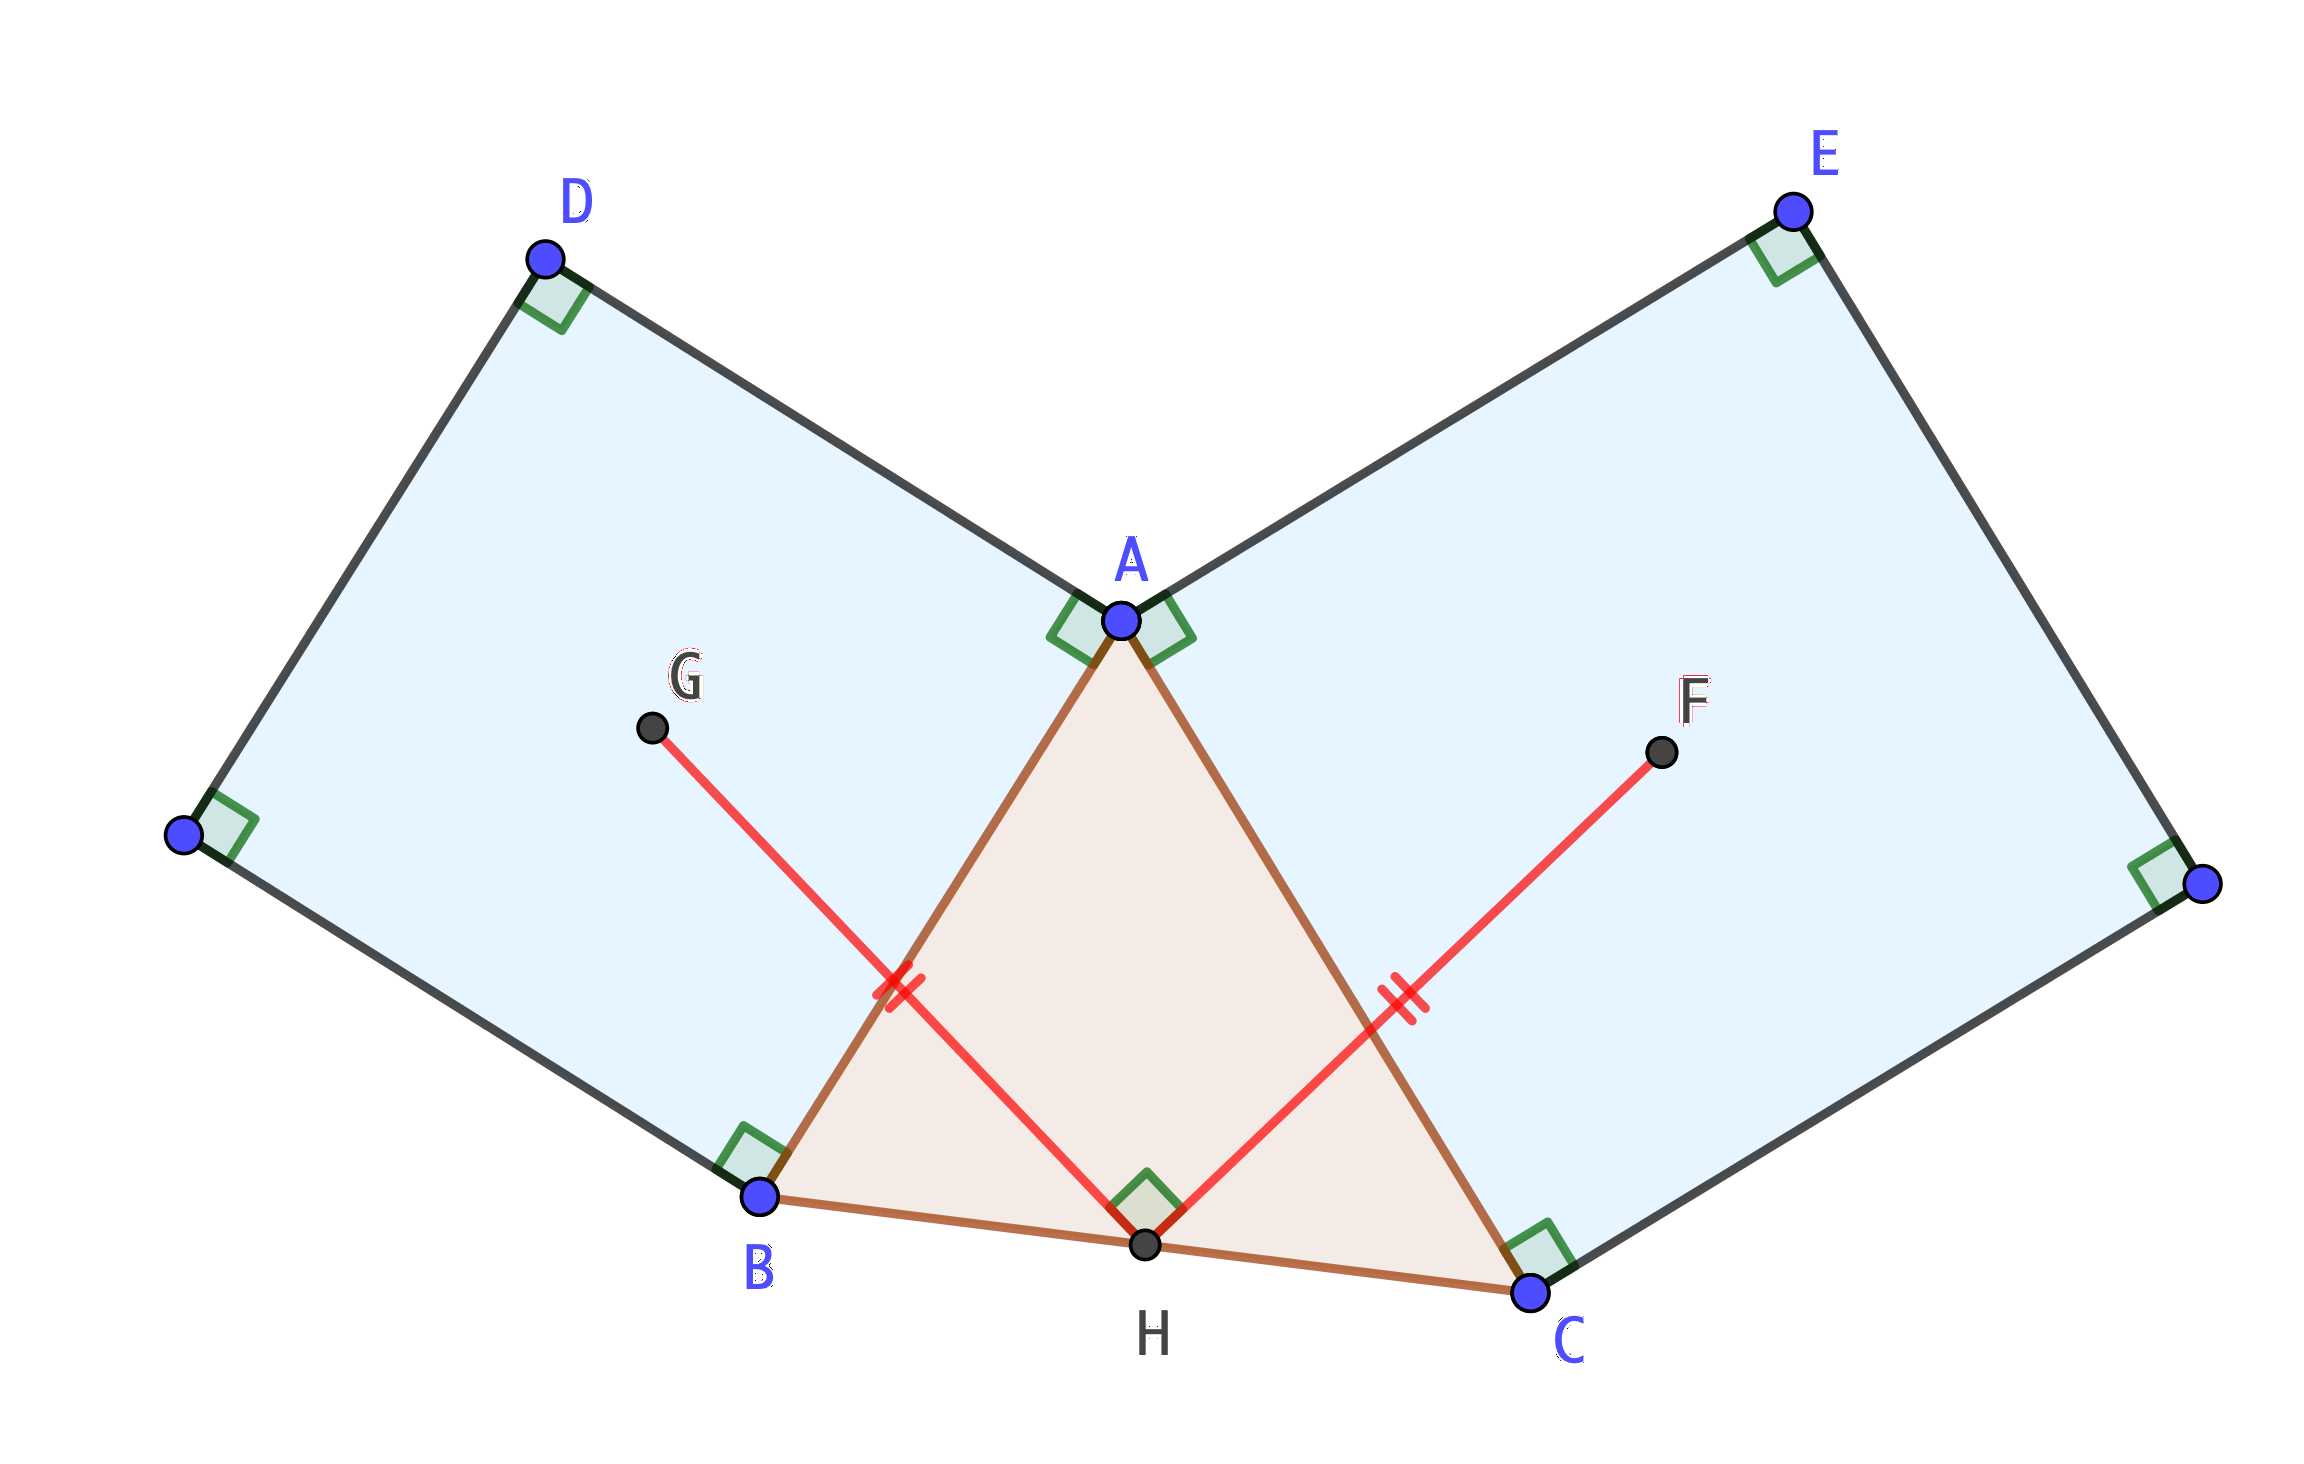
\includegraphics[scale=0.6]{kolmiotodistus.png}
\end{center}

\begin{proof}
Muodostetaan kolmiot ACD ja AEB. Koska sivut AC, EA ja AD, BA ovat keskenään yhtä suuret huomataan että muodostuneet kulmat $\measuredangle$DAC sekä $\measuredangle$BAE ovat molemmat suuruudeltaan $90^\circ + \alpha$, muodostetut kolmiot ovat yhtenevät. Tästä seuraa, että janat CD ja EB ovat yhtä pitkät.
\begin{center}
    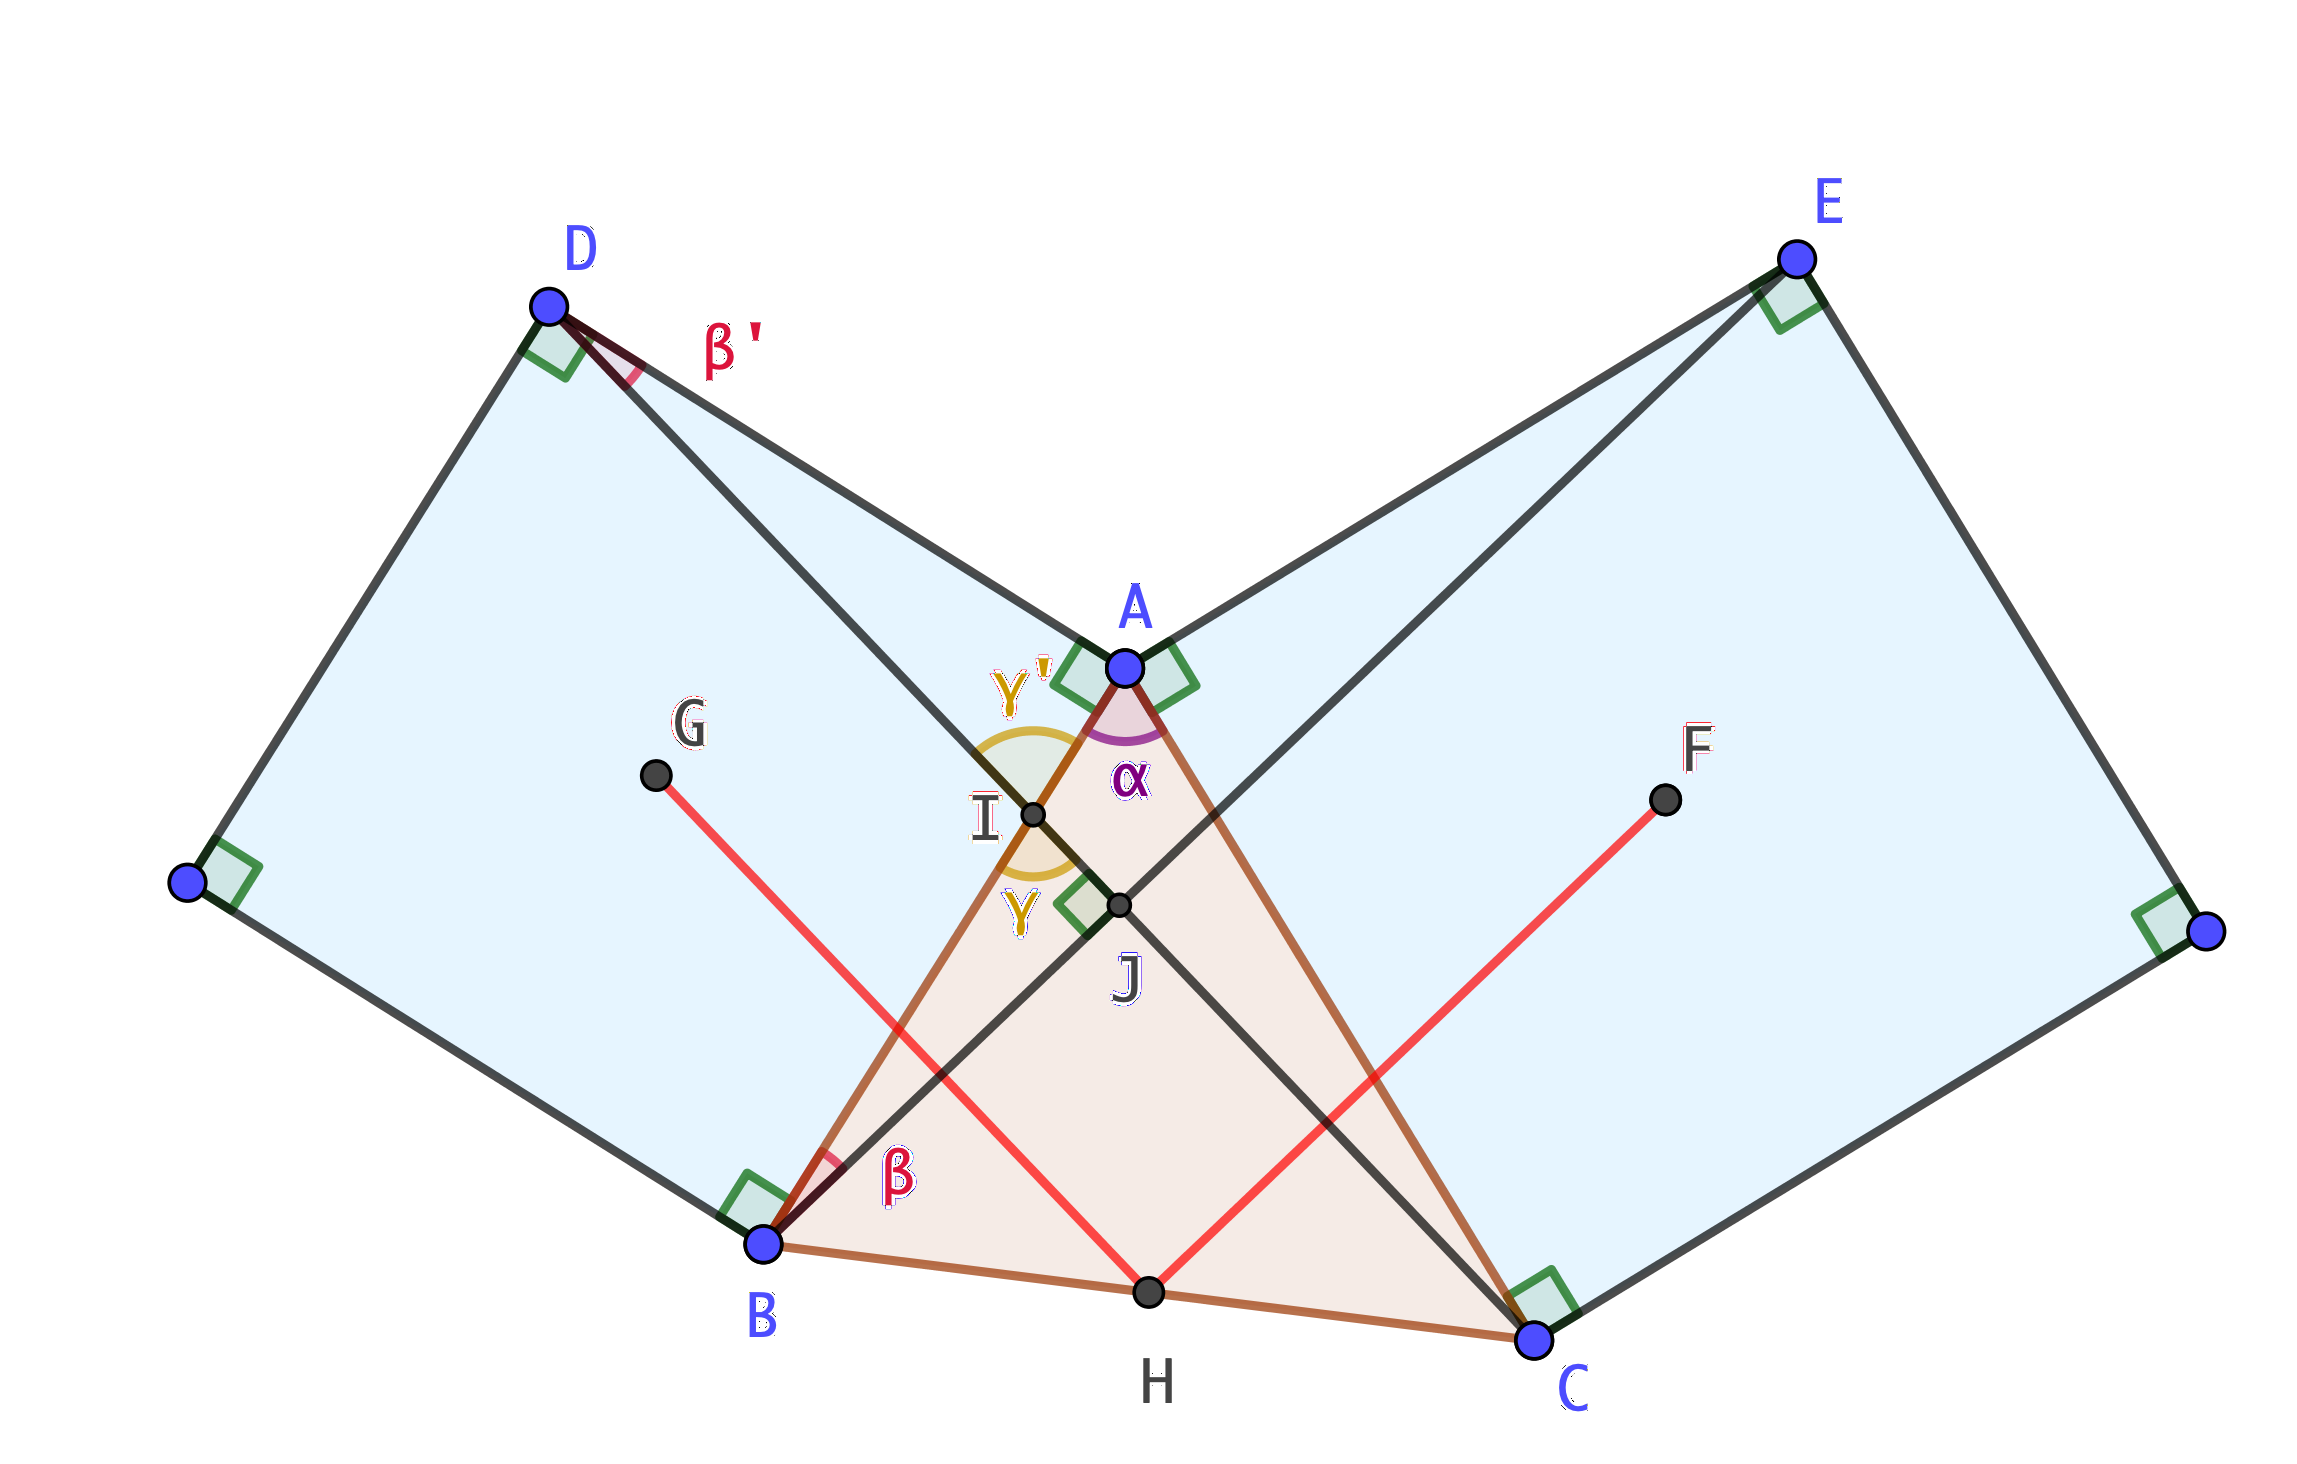
\includegraphics[scale=0.6]{kolmiojatkoa}
\end{center}

Yhtenevistä kolmioista seuraa myös se, että kulmat $\measuredangle$EBA ja $\measuredangle$CDA, nimetään ne $\beta$ ja $\beta'$, ovat yhtä suuret. Merkitään janojen CD ja BA leikkauspistettä pisteellä I. Huomataan myös, että kulmat $\measuredangle$BIJ ja $\measuredangle$AID ovat ristikulmia eli yhtä suuria, nimetään ne $\gamma$ ja $\gamma'$. Nyt sekä $\beta + \gamma = 90^\circ$ että $\beta' + \gamma' = 90^\circ$. Eli janat CD ja EB ovat kohtisuorassa toisiaan vastaan.

Muodostetaan kolmio CBD. Koska piste G on neliön lävistäjän keskipiste ja piste H on kolmion sivun keskipiste, muodostamme janan GH yhdistämällä näiden janojen keskipisteet janaksi GH. Tämän määritelmän mukaan janan GH pituus on CD/2 ja se on samansuuntainen janan CD kanssa. Sama huomataan kolmiosta CBE, eli jana HF muodostetaan yhdistämällä janojen EC ja CB janojen keskipisteet janaksi HF. Yhtälailla janan HF pituus on BE/2 ja se on samansuuntainen janan BE kanssa.

Ollaan aikaisemmin todistettu, että janat CD ja EB ovat yhtä pitkiä sekä kohtisuorassa toisiaan vastaan. Koska GH=CD/2 ja FH=EB/2 niin tällöin myös GH ja FH ovat yhtä pitkät. Ja koska janat BC ja EB ovat kohtisuorassa toisiaan vastaan ja janat GH ja FH ovat näiden kanssa samansuuntaiset eli janat GH ja FH ovat myös kohtisuorassa toisiaan vastaan eli niiden väliin muodostuu suora kulma.
\end{proof}


\pagebreak
\section{Todistus}
Lause voidaan todistaa joko vektorien tai geometrian avulla. Tässä esittelen todistuksen, joka on tehty geometrian avulla käyttäen yhteneviä kolmioita.

\medskip
\textbf{Lause:} Suorakulman sivuille piirretyistä neliöiden keskipisteistä yhdistetyt janat vastakkaiseen neliöön ovat yhtä pitkät ja toisiaan kohtaan kohtisuorassa. 
\begin{center}
    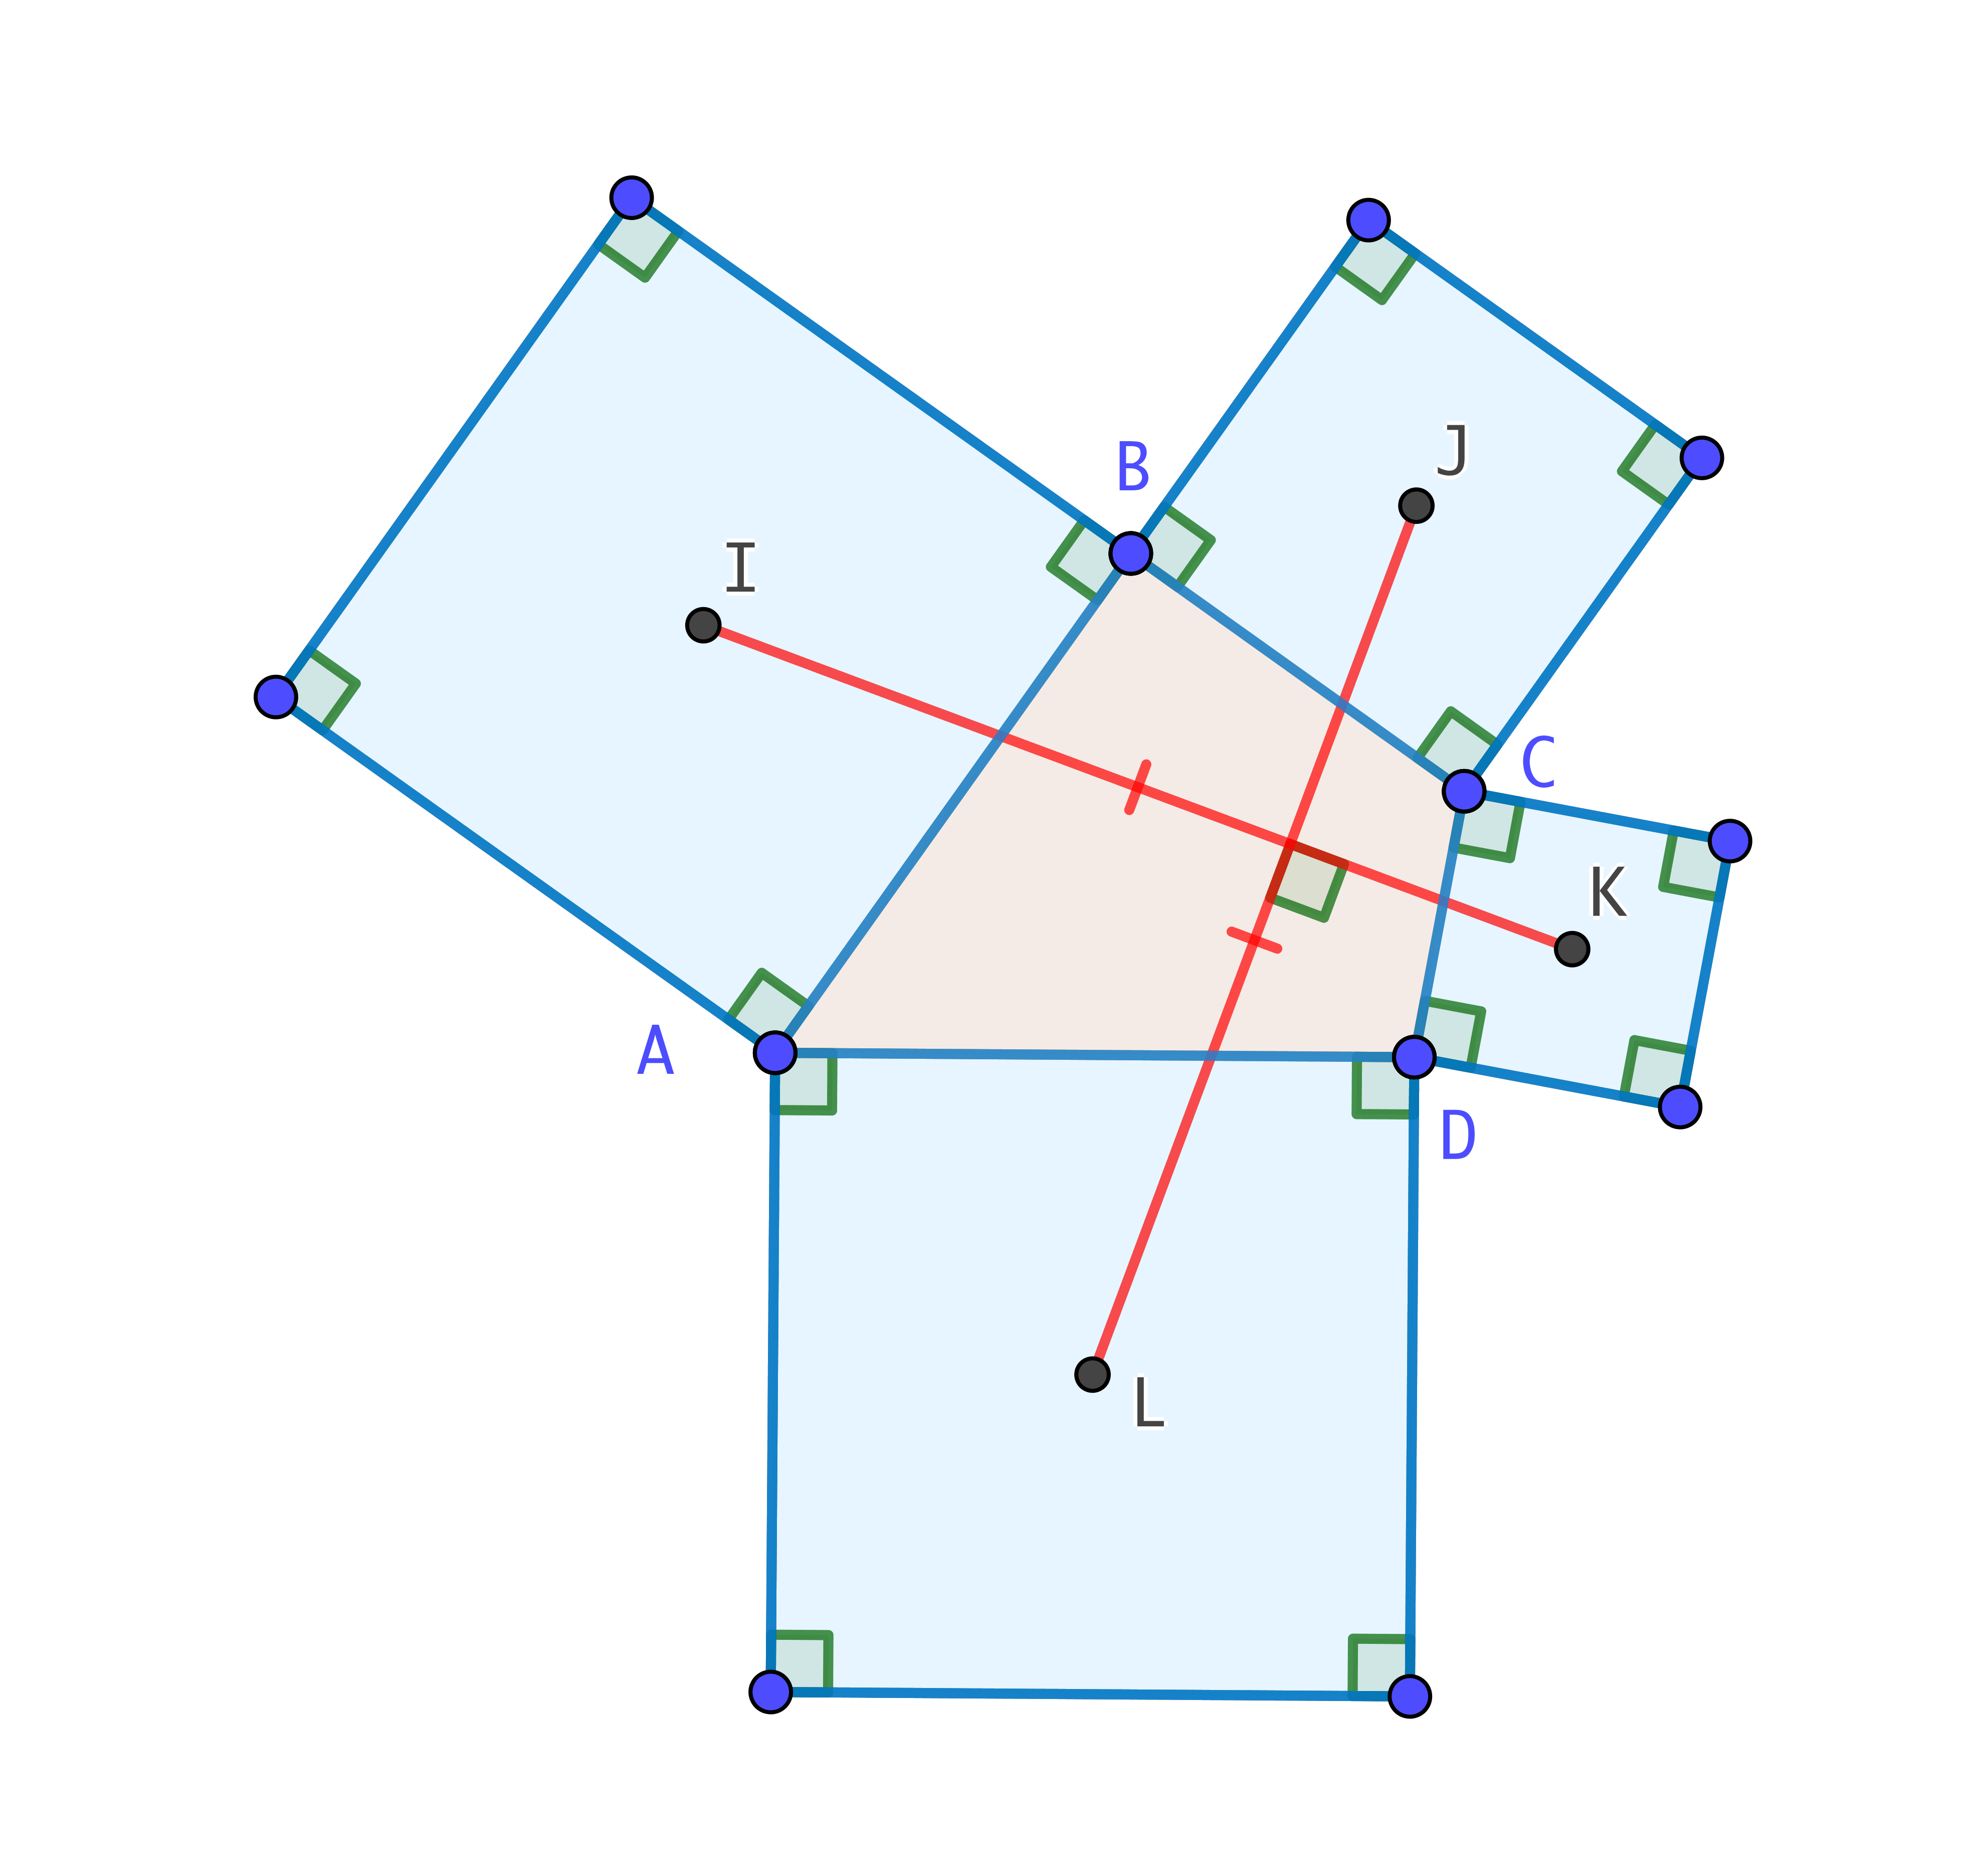
\includegraphics[scale=0.3]{todistuskuva}
\end{center}

Tämä lause pätee, vaikka nelikulmio ei olisi konveksi, jos nelikulmion yksi sivu kutistettaisiin pisteeksi sekä jos neliöt piirrettäisiin nelikulmion sisään. Todistan perustapauksen.

\medskip
\begin{proof}
Valitaan suorakulmion lävistäjältä AC keskipiste M. Piirretään janat IM ja JM. Nämä janat muodostavat suoran kulman aikaisemmin todistetun lauseen mukaan. Samoin muodostetaan janat LM ja KM, niillä on sama ominaisuus.
\begin{center}
    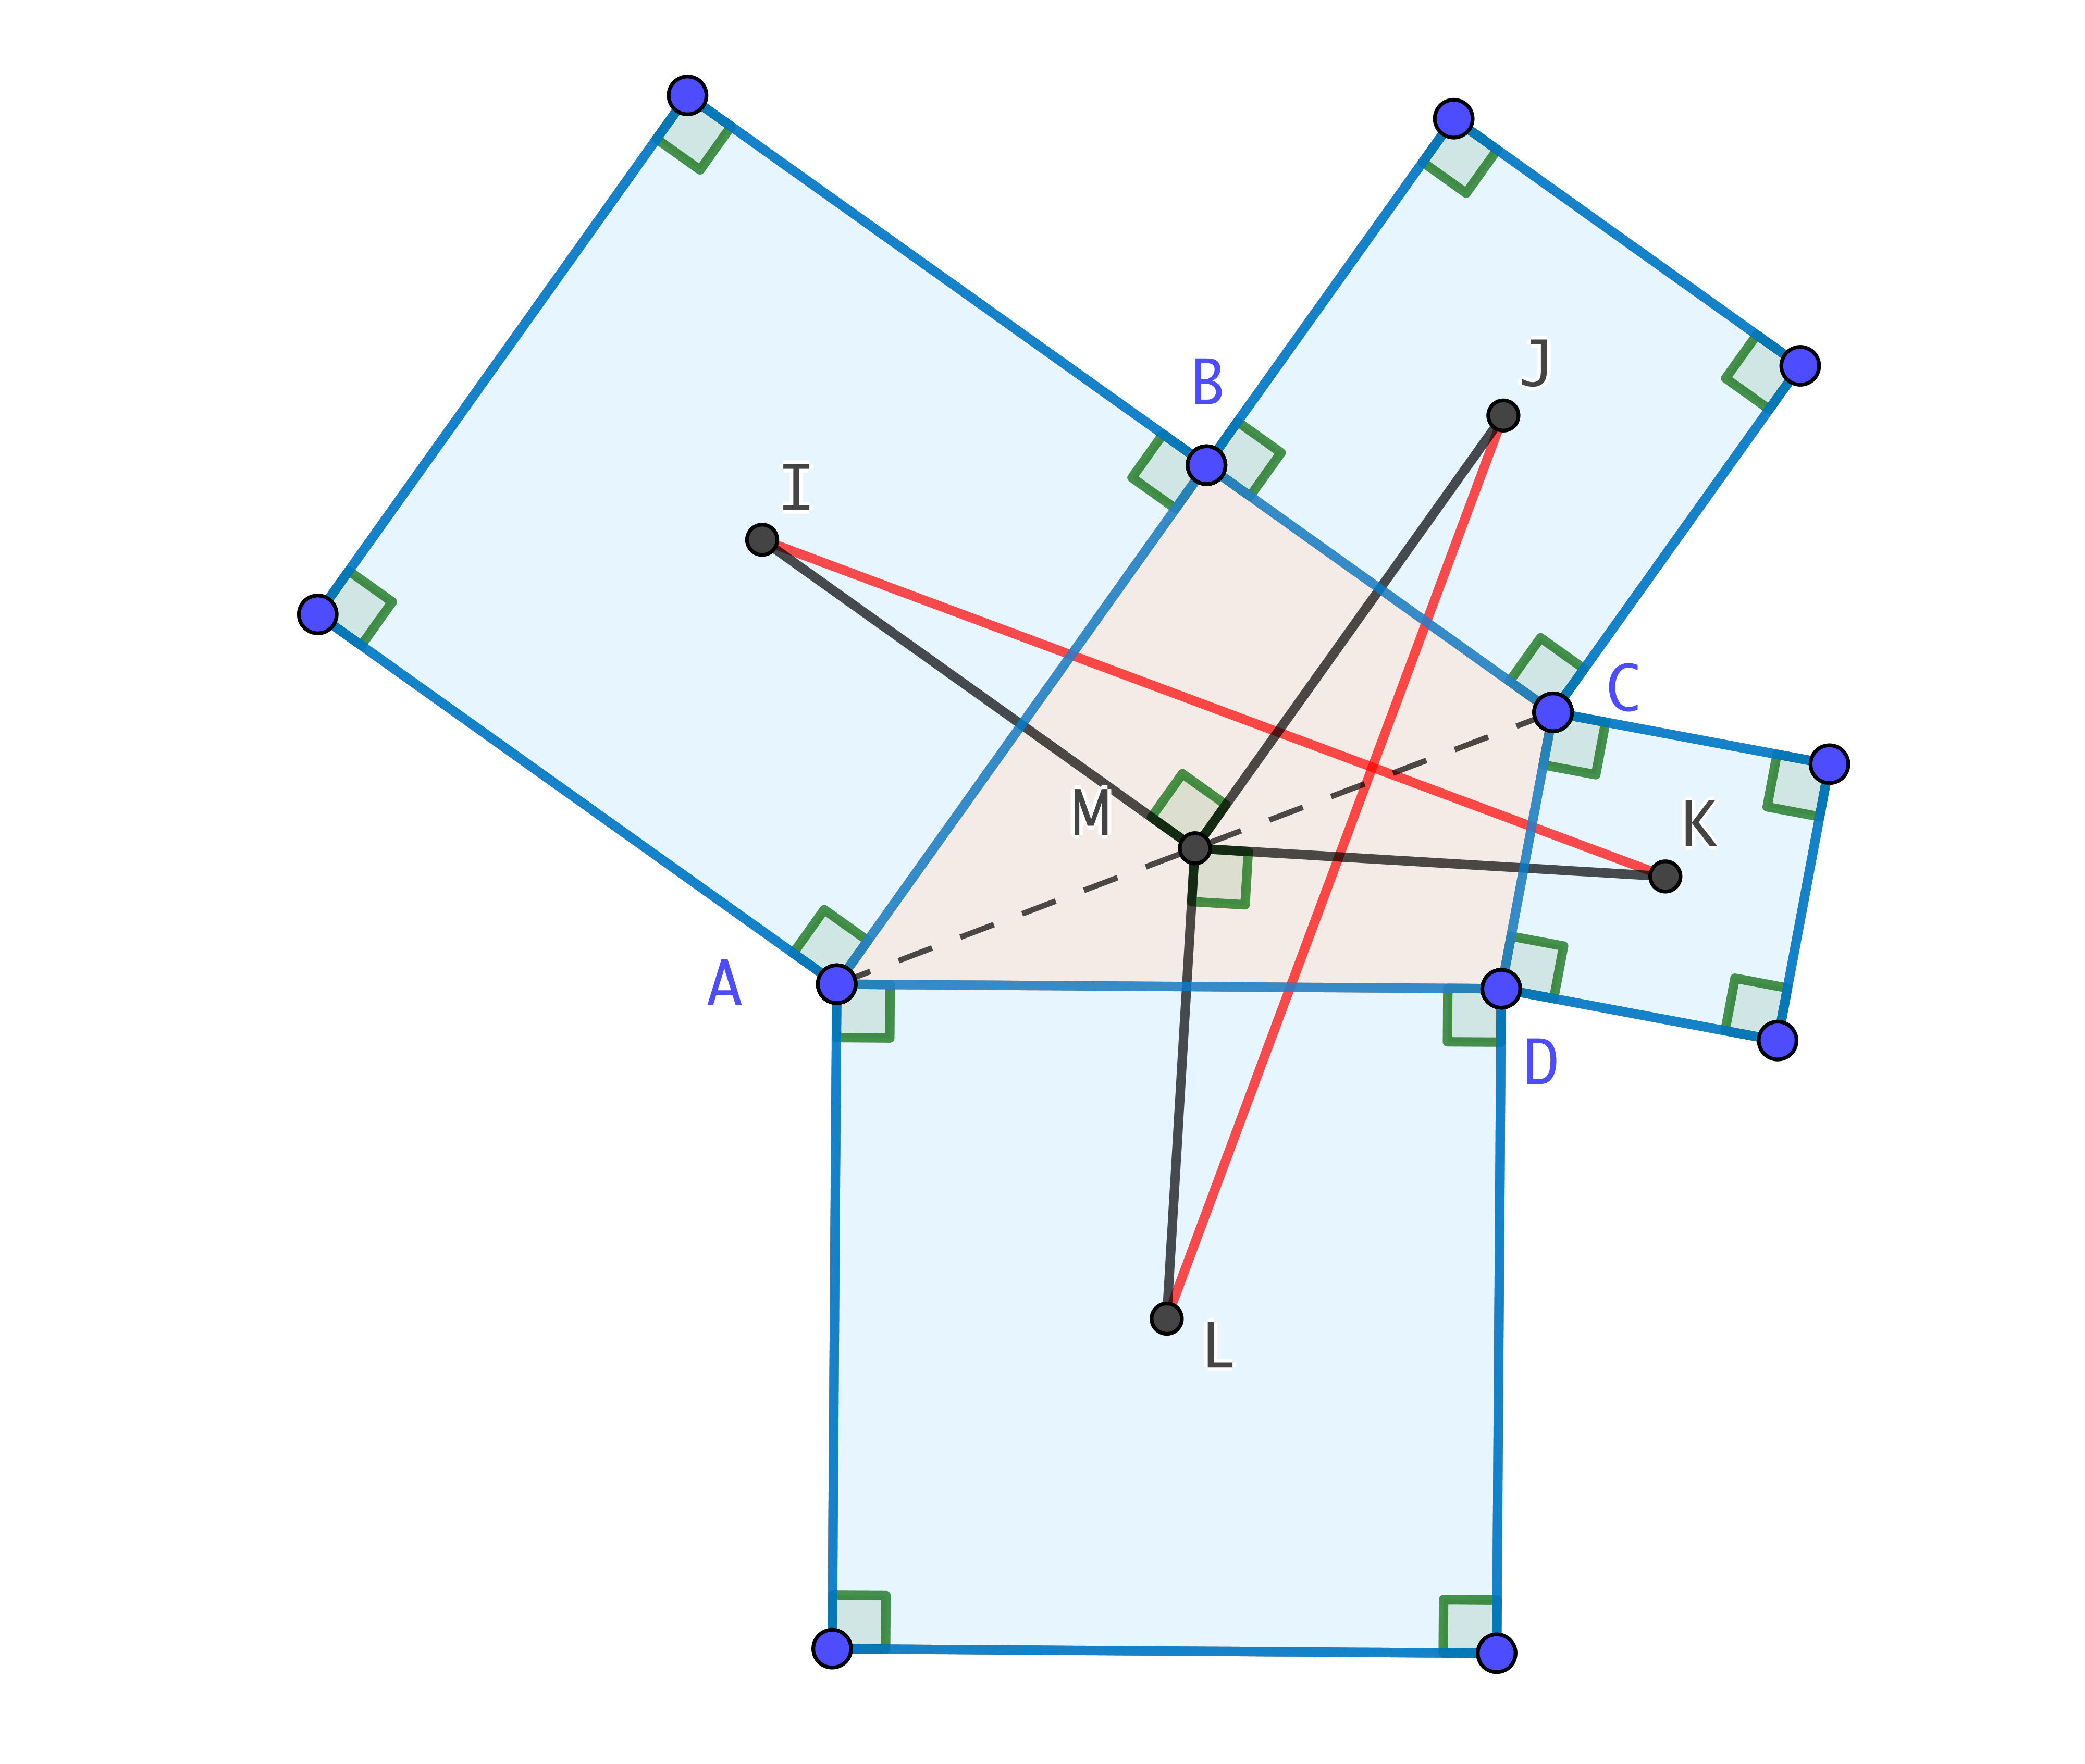
\includegraphics[scale=0.3]{todistus1}
\end{center}
Huomaamme, että kolmiot LMJ ja KMI ovat yhtenevät sillä molemmilla on kaksi samanpituista sivua IM, JM ja KM, LM, sekä niiden välillä suorakulma. Tästä seuraa, että sivut IK ja JL ovat myös yhtä pitkiä, näin ollaan todistettu osan lauseesta. Samaten siitä seuraa se että kulmat $\measuredangle$JLM ja $\measuredangle$IKM ovat yhtä suuret. Nimetään nämä kulmat $\alpha$ ja $\alpha'$.

Merkitään janojen JL ja KM leikkauspiste pisteellä N. Huomataan, että kulmat $\measuredangle$LNM ja $\measuredangle$JNK ovat ristikulmia eli yhtä suuret. Nimetään nämä kulmat $\beta$ ja $\beta'$.

\begin{center}
    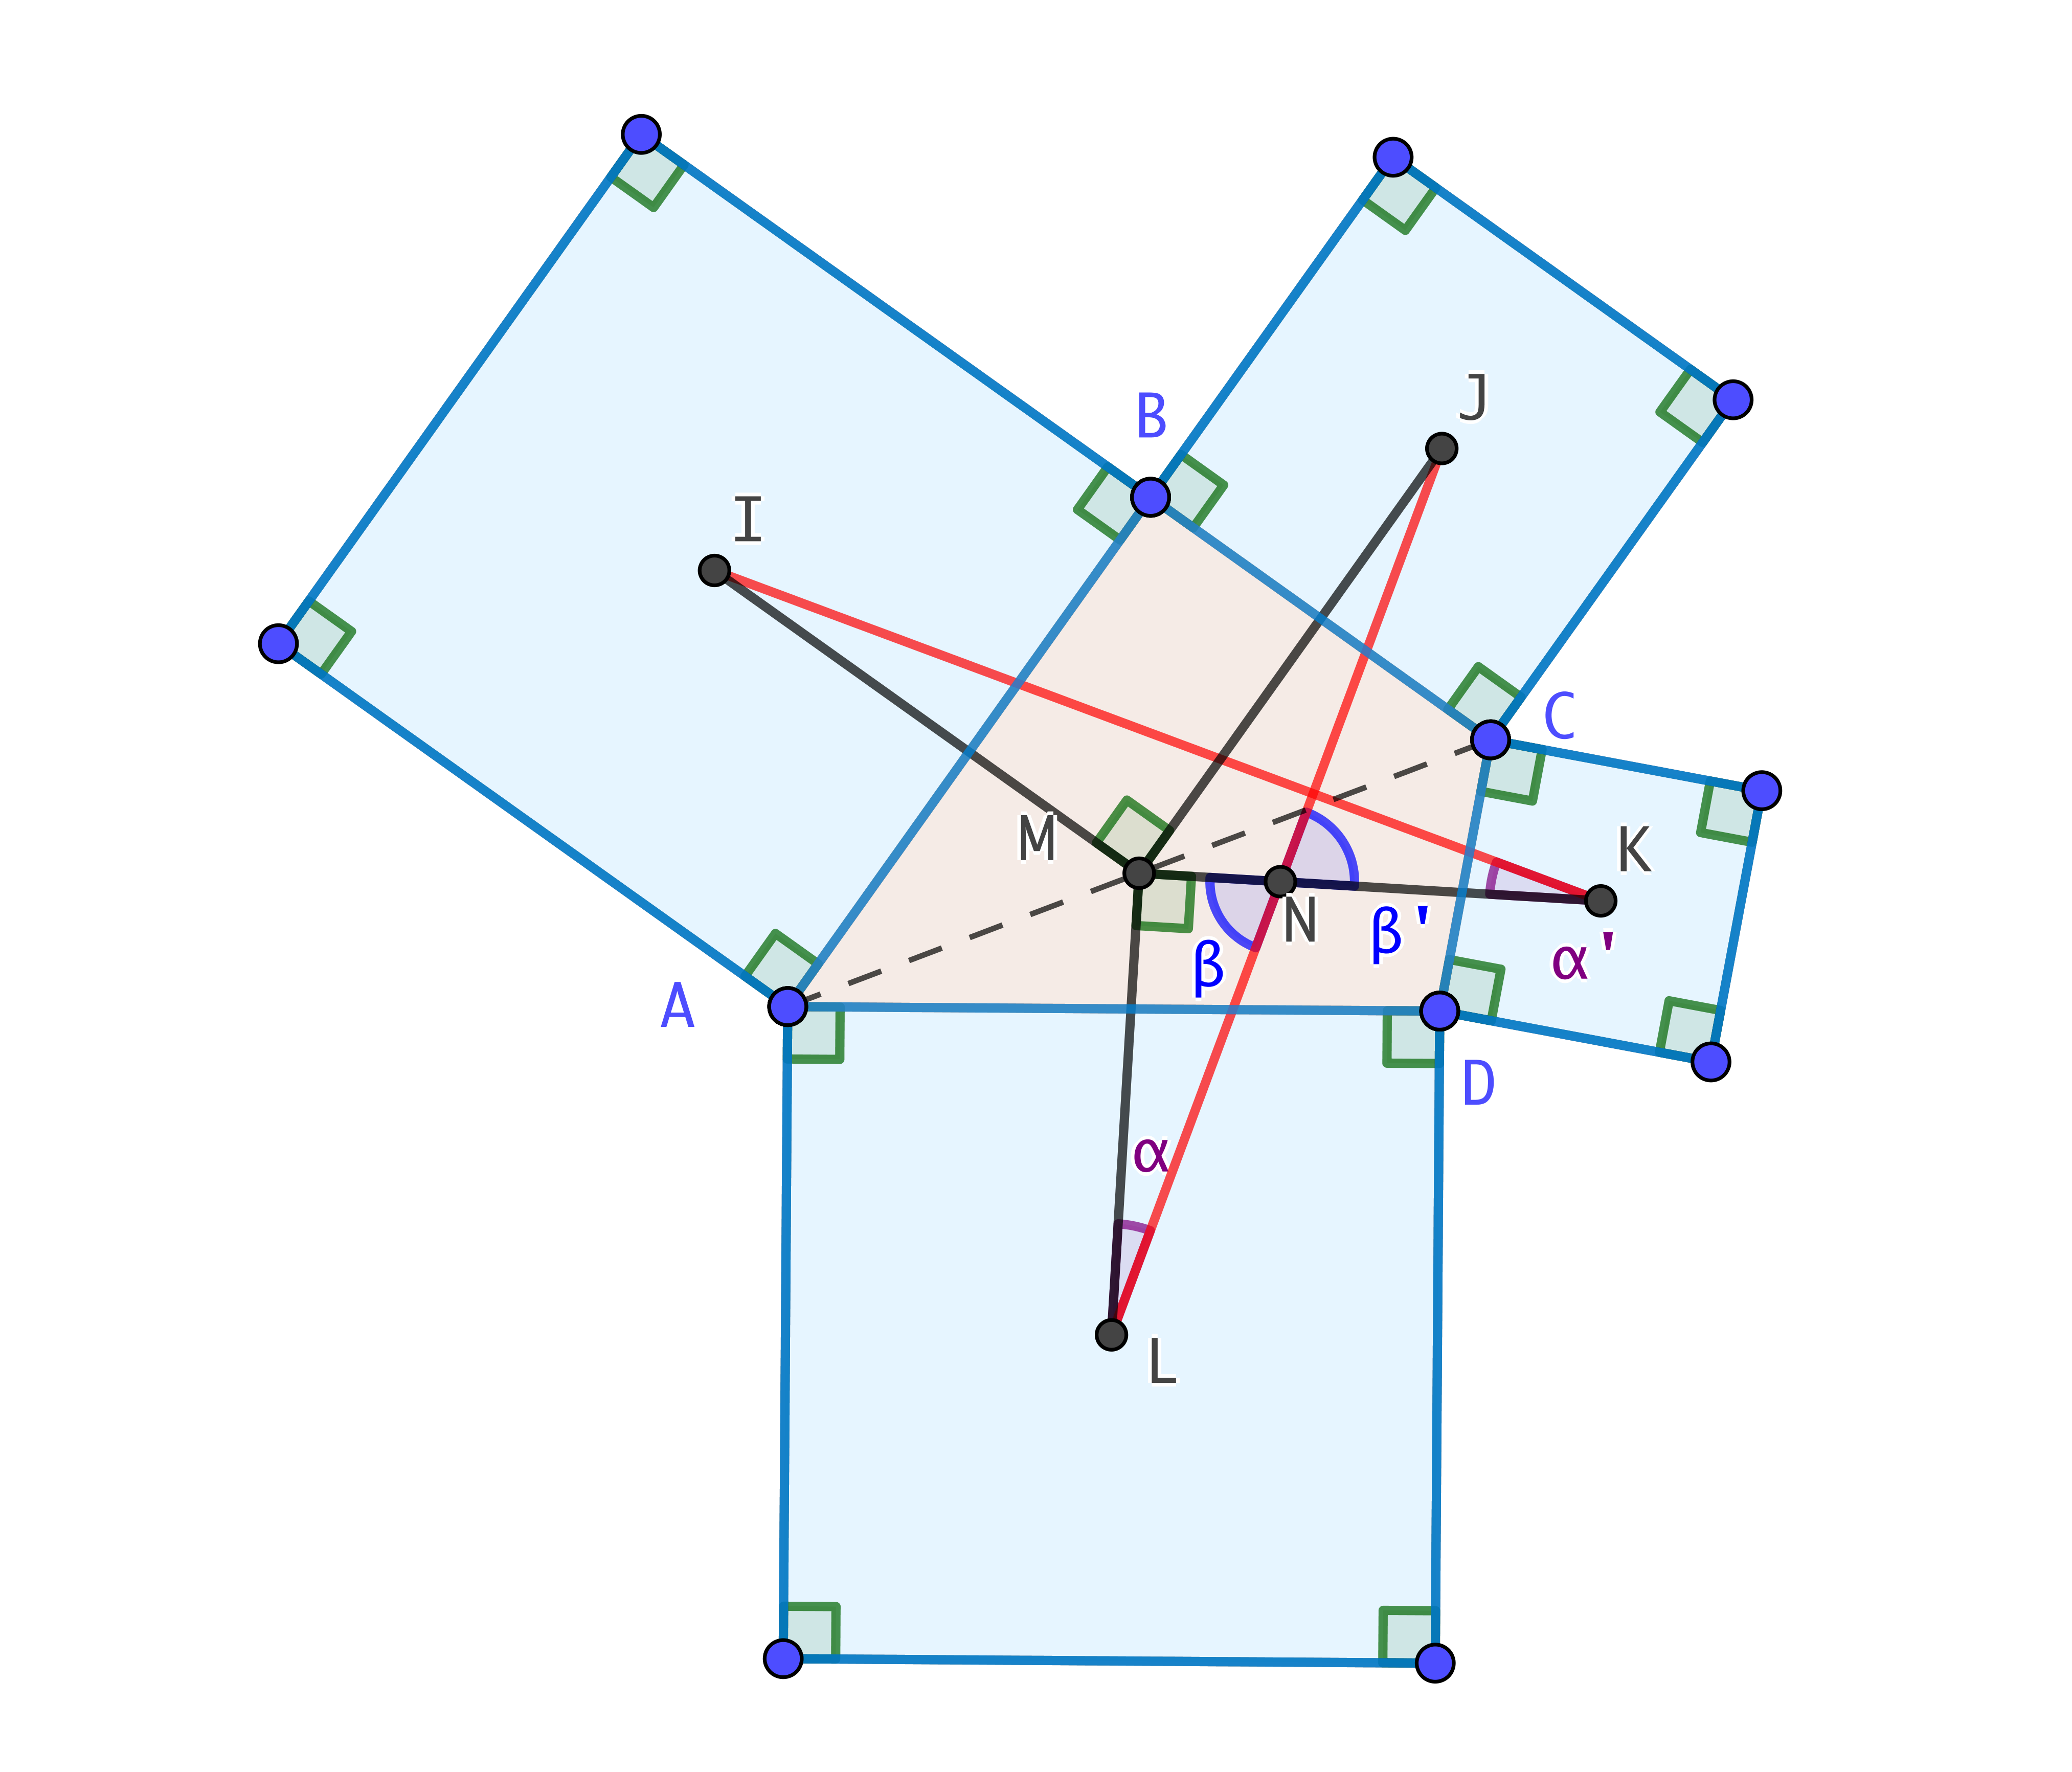
\includegraphics[scale=0.3]{todistuksenjatkoa.png}
\end{center}

Nyt nähdään, että $\alpha + \beta = 90^\circ$. Samaten myös $\alpha' + \beta' = 90^\circ$. Näin ollaan myös todistettu, että janat leikkaavat toisensa kohtisuorassa.
\end{proof}

\pagebreak
\section{Lauseen erikoistapaukset}
Alkuperäisessä van Aubelin todistuksessa ei todistettu muuta kuin, että janat ovat yhtä pitkät ja kohtisuorassa toisiaan vastaan. Lause pätee myös jos nelikulmion sivu kutistettaisiin pisteeksi.
\begin{center}
    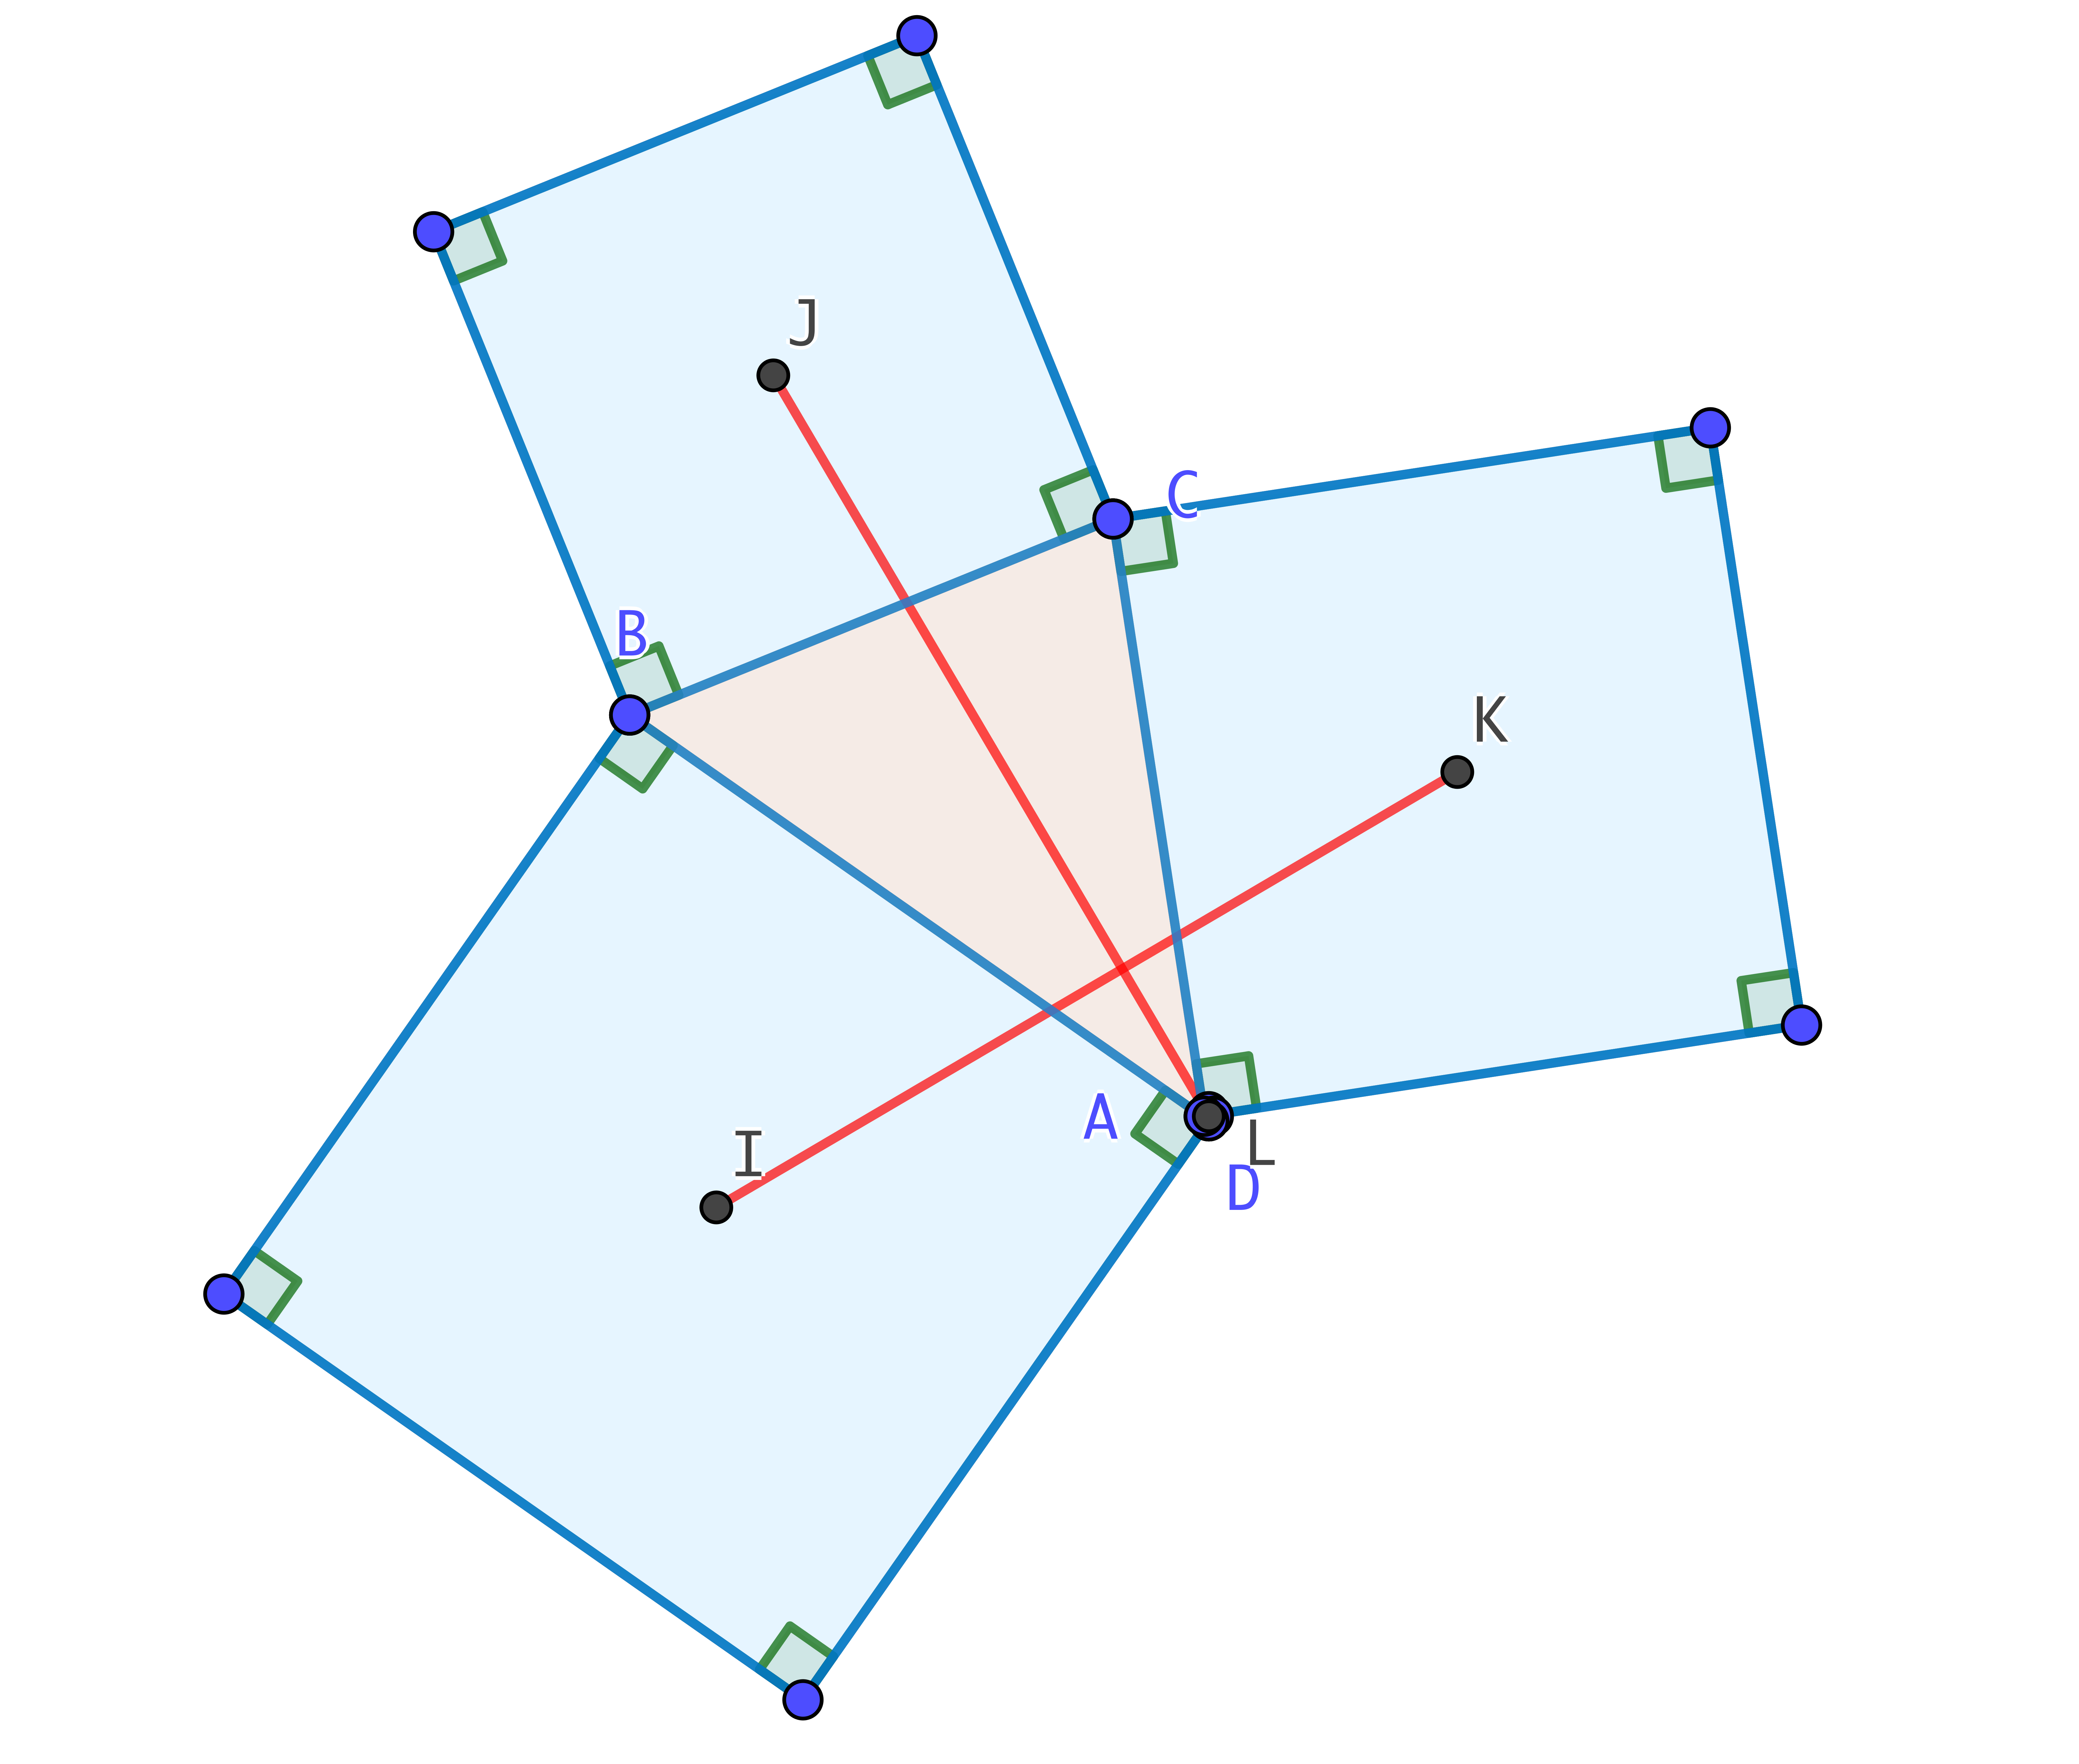
\includegraphics[scale=0.15]{sivupisteeksi.png}
\end{center}

Toinen erikoistapauks on jos nelikulmio leikkaa itsensä eli on kompleksinen. Tällöin janoja pidennetään puolisuoriksi jolloin ne leikkaavat toisensa jossain vaiheessa, mutta neliöiden keskipisteitä yhdistävät janat pysyvät edelleen yhtä pitkinä.
\begin{center}
    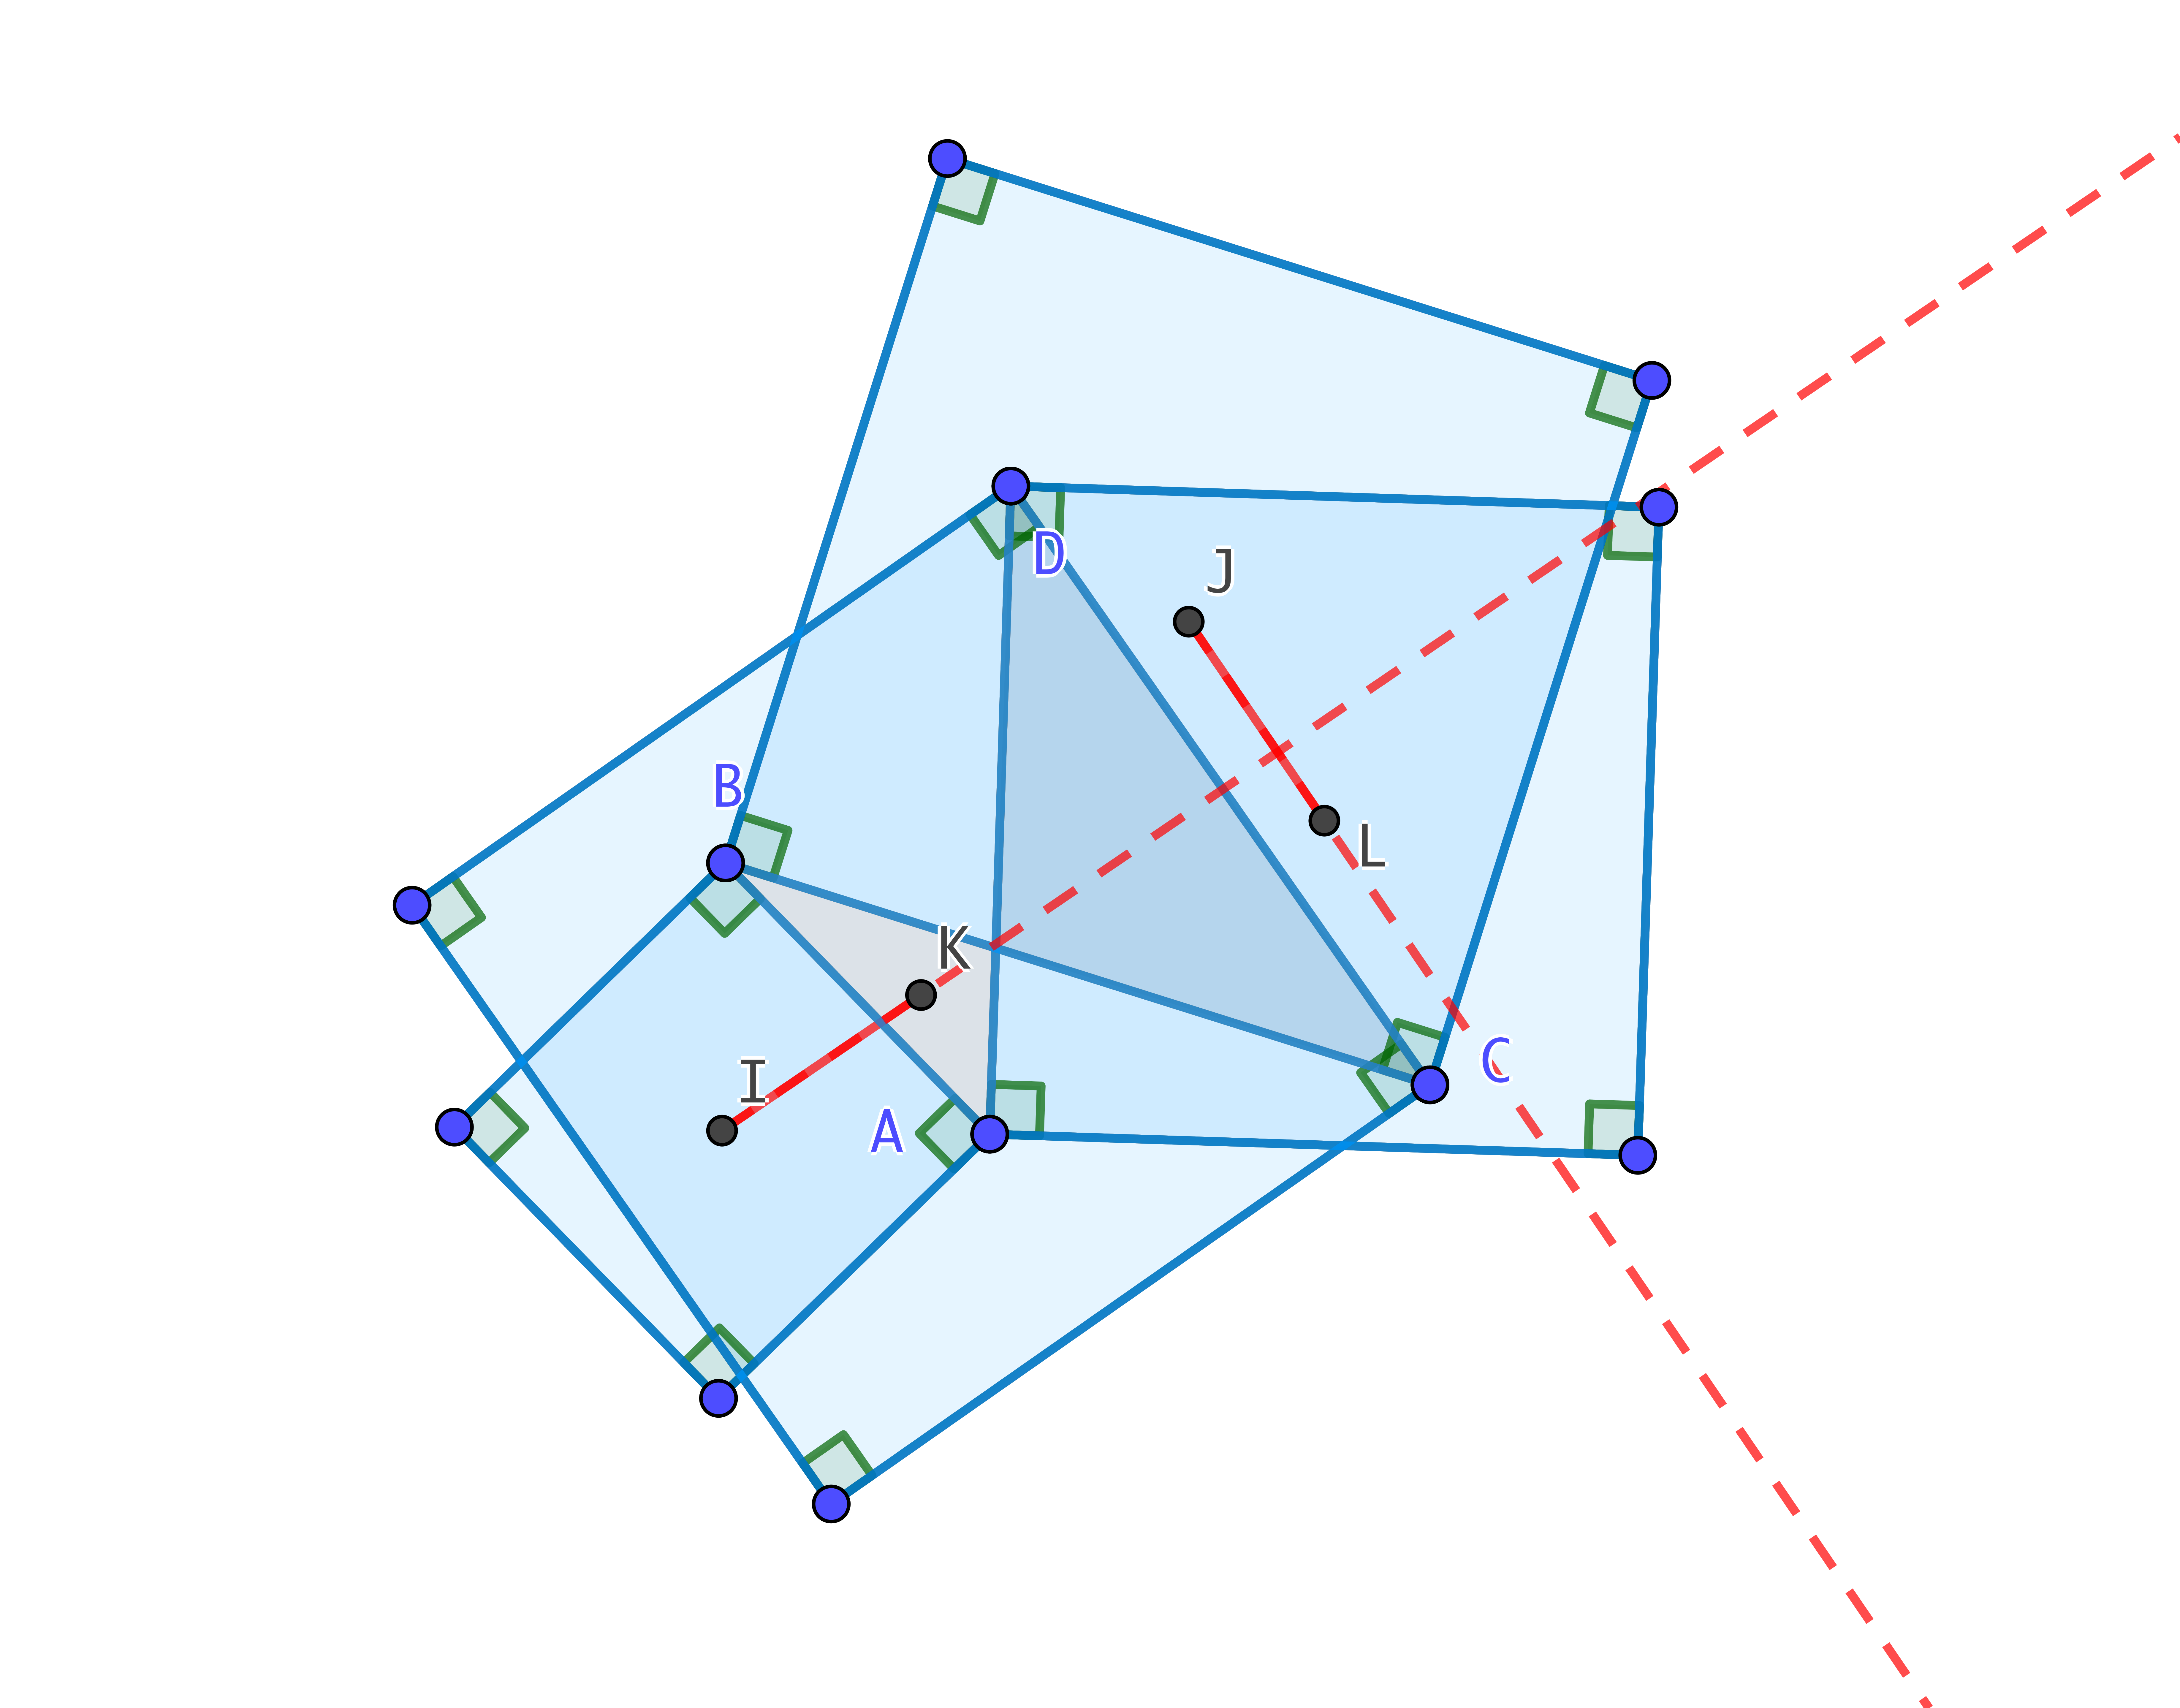
\includegraphics[scale=0.15]{konveksi.png}
\end{center}

Kolmas erikoistapaus, jossa lause pitää paikkansa on jos neliöt piirretään nelikulmion sisään eikä sen ulkopuolelle. 

Tämän lisäksi lauseella on muitakin ominaisuuksia, kuten se, jos neliöiden keskipisteet yhdistetään vierekkäisten neliöiden keskipisteiden kanssa, syntynyt nelikulmio on ortadiagonaalinen nelikulmio eli sen lävistäjät leikkaavat toisensa kohtisuorassa.
\begin{center}
    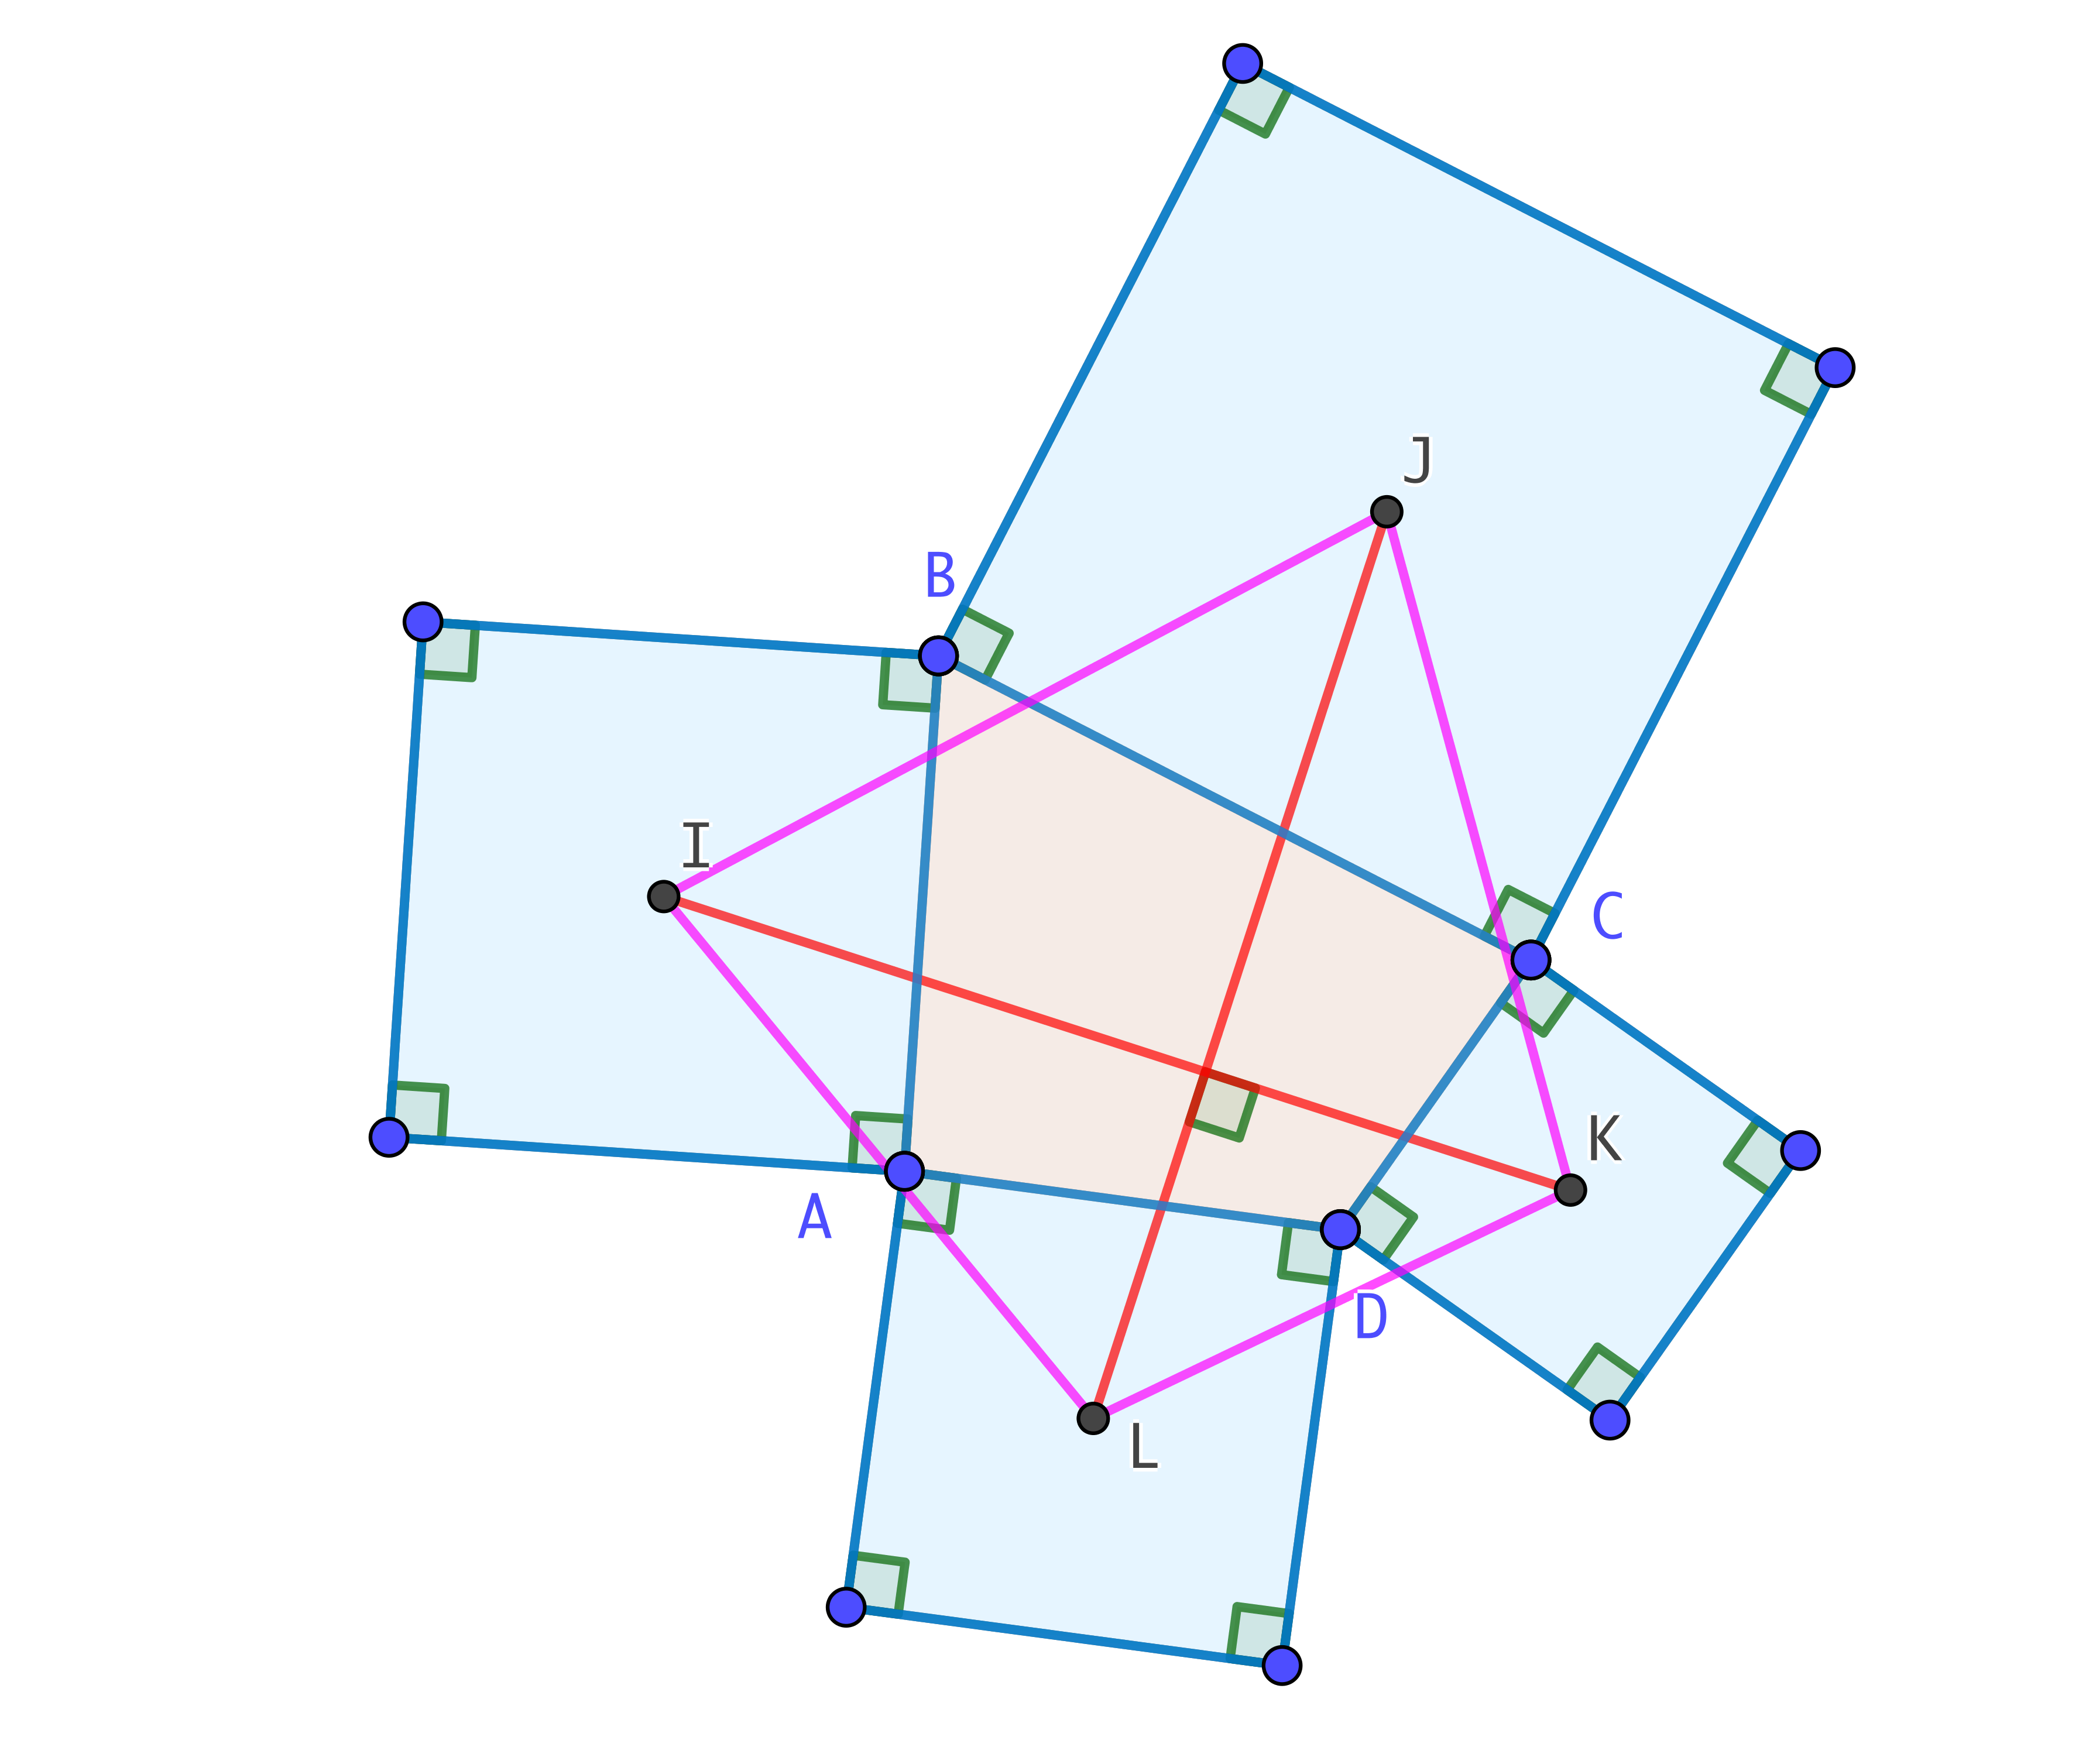
\includegraphics[scale=0.3]{ortadiagonaali.png}
\end{center}


\pagebreak
\section{Viitteitä muihin lauseisiin}
%http://mathworld.wolfram.com/vanAubelsTheorem.html

Van Aubelin lauseen tapaisia lauseita ovat muun muassa Napoleonin lause, Thebaultin teoreema sekä Petr–Douglas–Neumann teoreema.

Napoleonin lause todistaa, että jos jonkin kolmion sivuihin piirretään tasasivuiset kolmiot, samalla tyylillä kuin van Aubelin lauseessa, niin kun yhdistetään kolmioiden painopisteet keskenään muodostuu uusi tasasivuinen kolmio.
\begin{center}
    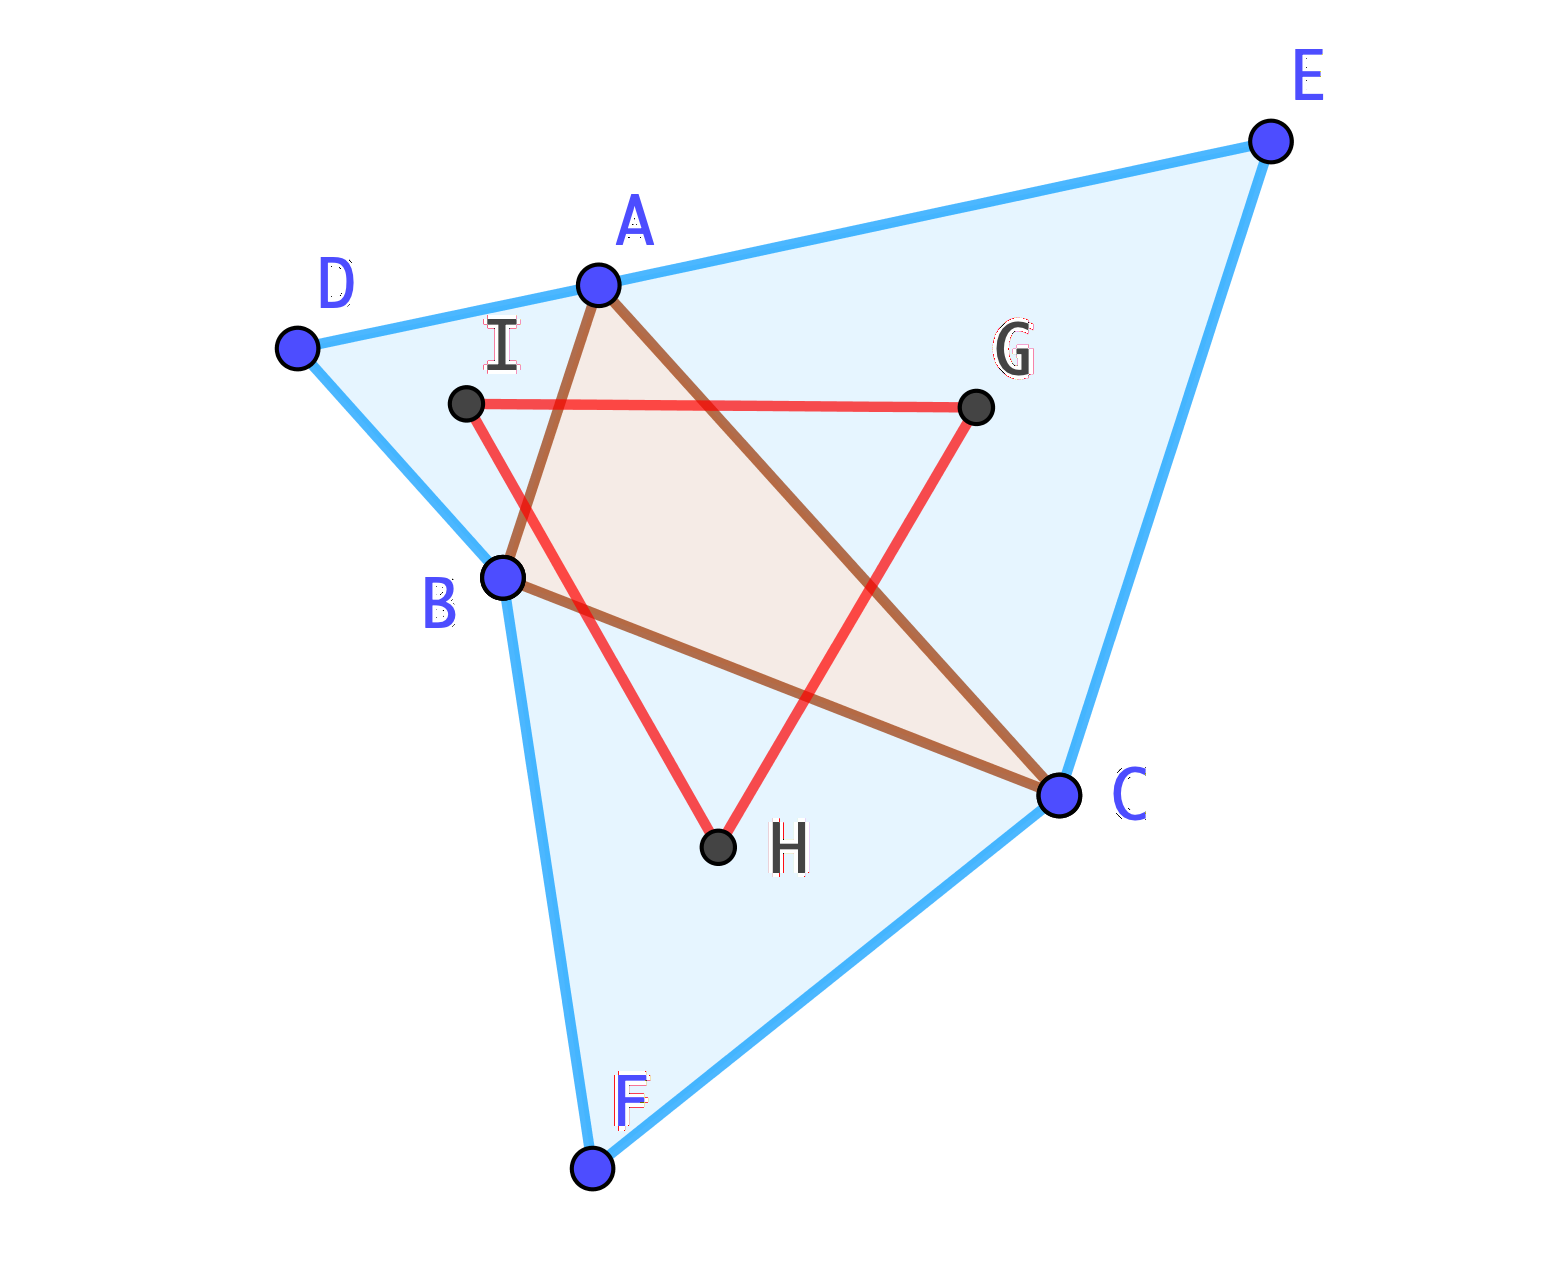
\includegraphics[scale=0.6]{Napoleonin.png}
\end{center}

Thebaultin teoreemoja on kolme. Näistä ensimmäinen teoreema on van Aubelin lauseen erikoistapaus. Sen mukaan jos alkuperäinen nelikulmio on suunnikas ja sen reunoihin piirretään neliöt, tällöin vierekkäisten neliöiden keskipisteitä yhdistäessä muodostuu uusi neliö.

Petr–Douglas–Neumann teoreema 


\pagebreak
\section{Lähteet}
%van Aubel, H. H. (1878), "Note concernant les centres de carrés construits sur les côtés d'un polygon quelconque", Nouvelle Correspondance Mathématique (In French), 4: 40–44.

%http://www.osaka-ue.ac.jp/zemi/nishiyama/math2010/aubel.pdf

%http://mathworld.wolfram.com/vanAubelsTheorem.html

\end{document}